\documentclass[12pt]{article}
\usepackage[utf8]{inputenc}
\usepackage[T1]{fontenc} % uses T1 fonts (better quality)
\usepackage{lmodern} % uses Times fonts
% \usepackage{mathptmx} % uses Times fonts
% \mathrm = un-italicize math fonts
\usepackage[dvipsnames]{xcolor}
\usepackage[margin=1in]{geometry}
% \usepackage{nopageno} % no page numbers
\usepackage{graphicx}
\usepackage{pdfpages}
\usepackage{bm}
\graphicspath{ {./img/} }
\usepackage{booktabs}   % for table borders
\usepackage{amsmath}
\usepackage[makeroom]{cancel}
\usepackage{tikz}
\usetikzlibrary{shapes,arrows}

\begin{document}
 	\begin{center}
    \line(1,0){300}\\[0.25cm]
 	\Large{\bfseries ECE540: Homework \#2}\\
 	\textsc{\large David Kirby}\\
 	\textsc{\large Due: 24 September 2020}\\
 	\line(1,0){300}\\[0.75cm]
 	\end{center}

% Define block styles
% \tikzstyle{decision} = [diamond, draw, fill=blue!20,
%     text width=4.5em, text badly centered, node distance=3cm, inner sep=0pt]
\tikzstyle{block} = [rectangle, draw,
    text width=20em, text centered, rounded corners, minimum height=1em]
\tikzstyle{line} = [draw, -latex']
\tikzstyle{cloud} = [draw, ellipse,fill=red!20, node distance=3cm,
    minimum height=2em]
Chapter 6: R3, R6, R9, R11, P8, P9, P12, P13, P14, P21, P22, P29, P33.

\section*{Chapter 6}
\subsection*{Review Questions}
\begin{enumerate}
\item R3. Name three error-detection strategies employed by link layer.

\item R6. In CSMA/CD, after the fifth collision, what is the probability that a node
chooses \(K = 4\)? The result \(K = 4\) corresponds to a delay of how many seconds on a 10 Mbps Ethernet?

\item R9. How big is the MAC address space? The IPv4 address space? The IPv6
address space?

\item R11. Why is an ARP query sent within a broadcast frame? Why is an ARP
response sent within a frame with a specific destination MAC address?
\end{enumerate}
\subsection*{Problems}
\begin{enumerate}
    \item P8. In Section 6.3, we provided an outline of the derivation of the efficiency of slotted ALOHA.\ In this problem we’ll complete the derivation.
    \begin{enumerate}
        \item Recall that when there are \textit{N} active nodes, the efficiency of slotted ALOHA is \(Np{(1 - p)}^{N-1}\). Find the value of \textit{p} that maximizes this expression.
        \item Using the value of \textit{p} found in (a), find the efficiency of slotted ALOHA by letting \textit{N} approach infinity. \textit{Hint}: \({(1 - 1/N)}^N\) approaches \(1/e\) as \textit{N} approaches infinity.
    \end{enumerate}
    \item P9. Show that the maximum efficiency of pure ALOHA is \(1/(2e)\). \textit{Note}: This problem is easy if you have completed the problem above!
    \item P12. Graph the efficiency of slotted ALOHA and pure ALOHA as a function of \textit{p} for the following values of \textit{N}:
    \begin{enumerate}
        \item \(N=15\).
        \item \(N=25\).
        \item \(N=35\).
    \end{enumerate}
    \item P13. Consider a broadcast channel with \textit{N} nodes and a transmission rate of \text{R} bps. Suppose the broadcast channel uses polling (with an additional polling node) for multiple access. Suppose the amount of time from when a node completes transmission until the subsequent node is permitted to transmit (that is, the polling delay) is \(d_{\mathrm{poll}}\). Suppose that within a polling round, a given node is allowed to transmit at most \textit{Q} bits. What is the maximum throughput of the broadcast channel?
    \item P14. Consider three LANs interconnected by two routers, as shown in Figure 6.33.
    \begin{figure}[h!]
        \centering
        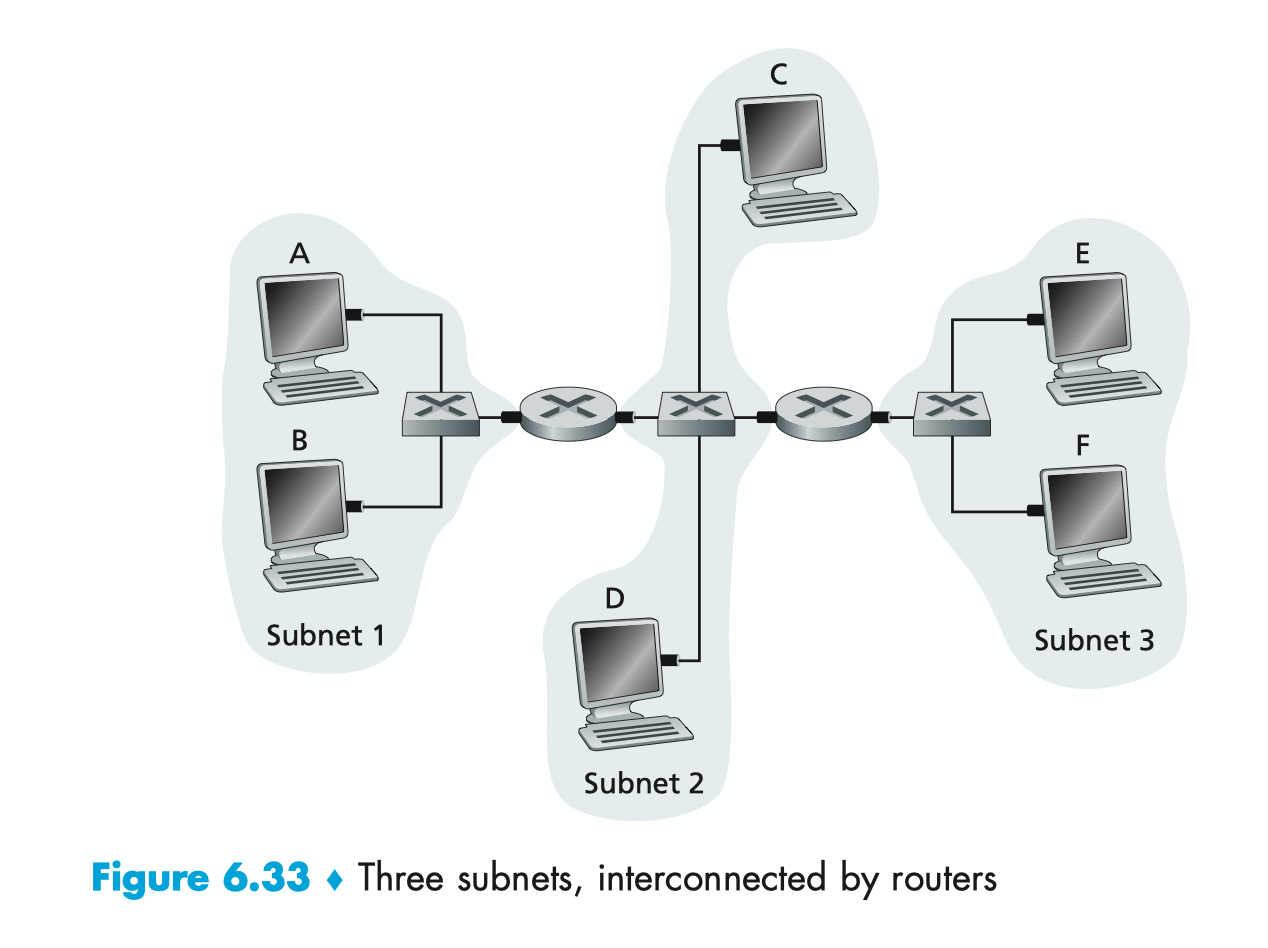
\includegraphics[width=0.85\textwidth]{Fig6.33.png}
        % \caption{}
        % \label{fig:I2Cdemo}
    \end{figure}
    \begin{enumerate}
        \item Assign IP addresses to all of the interfaces. For Subnet 1 use addresses of the form 192.168.1.xxx; for Subnet 2 uses addresses of the form 192.168.2.xxx; and for Subnet 3 use addresses of the form 192.168.3.xxx.
        \item Assign MAC addresses to all of the adapters.
        \item Consider sending an IP datagram from Host E to Host B. Suppose all of the ARP tables are up to date. Enumerate all the steps, as done for the single-router example in Section 6.4.1.
        \item Repeat (c), now assuming that the ARP table in the sending host is empty (and the other tables are up to date).
    \end{enumerate}
    \item P21. Consider Figure 6.33 in problem P14. Provide MAC addresses and IP addresses for the interfaces at Host A, both routers, and Host F. Suppose Host A sends a datagram to Host F. Give the source and destination MAC addresses in the frame encapsulating this IP datagram as the frame is transmitted \textit{(i)} from A to the left router, \textit{(ii)} from the left router to the right router, \textit{(iii)} from the right router to F. Also give the source and destination IP addresses in the IP datagram encapsulated within the frame at each of these points in time.
    \item P22. Suppose now that the leftmost router in Figure 6.33 is replaced by a switch. Hosts A, B, C, and D and the right router are all star-connected into this switch. Give the source and destination MAC addresses in the frame encapsulating this IP datagram as the frame is transmitted \textit{(i)} from A to the switch, \textit{(ii)} from the switch to the right router, \textit{(iii)} from the right router to F. Also give the source and destination IP addresses in the IP datagram encapsulated within the frame at each of these points in time.
    \item P29. Consider the MPLS network shown in Figure 6.29, and suppose that routers R5 and R6 are now MPLS enabled. Suppose that we want to perform traffic engineering so that packets from R6 destined for A are switched to A via R6-R4-R3-R1, and packets from R5 destined for A are switched via R5-R4-R2-R1. Show the MPLS tables in R5 and R6, as well as the modified table in R4, that would make this possible.
    \begin{figure}[h!]
        \centering
        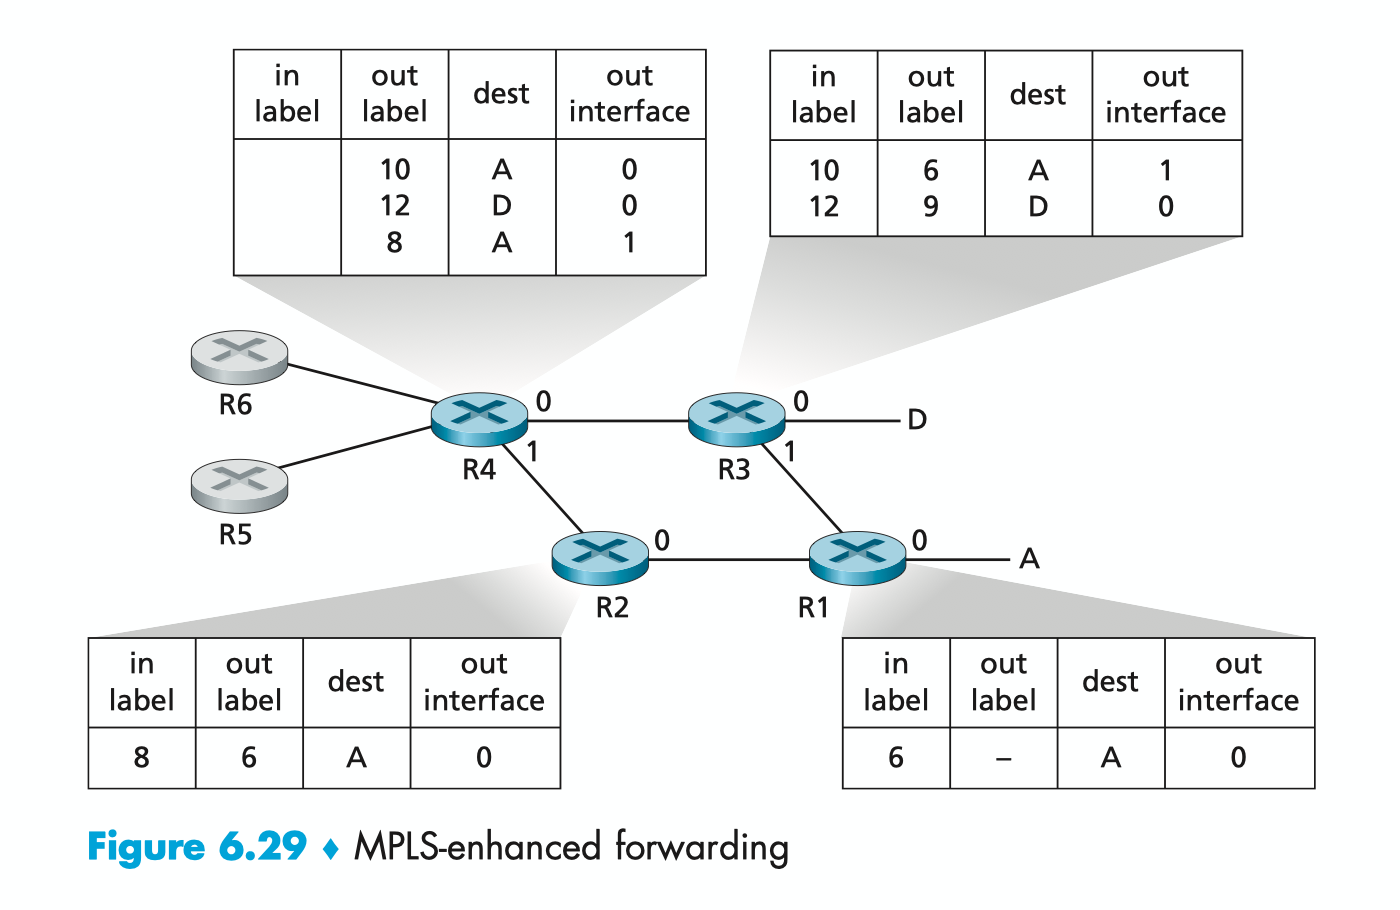
\includegraphics[width=0.85\textwidth]{Fig6.29.png}
        % \caption{}
        % \label{fig:I2Cdemo}
    \end{figure}
    \item P33. Consider the hierarchical network in Figure 6.30 and suppose that the data center needs to support e-mail and video distribution among other applications. Suppose four racks of servers are reserved for e-mail and four racks are reserved for video. For each of the applications, all four racks must lie below a single tier-2 switch since the tier-2 to tier-1 links do not have sufficient bandwidth to support the intra-application traffic. For the e-mail application, suppose that for 99.9 percent of the time only three racks are used, and that the video application has identical usage patterns.
    \begin{figure}[h!]
        \centering
        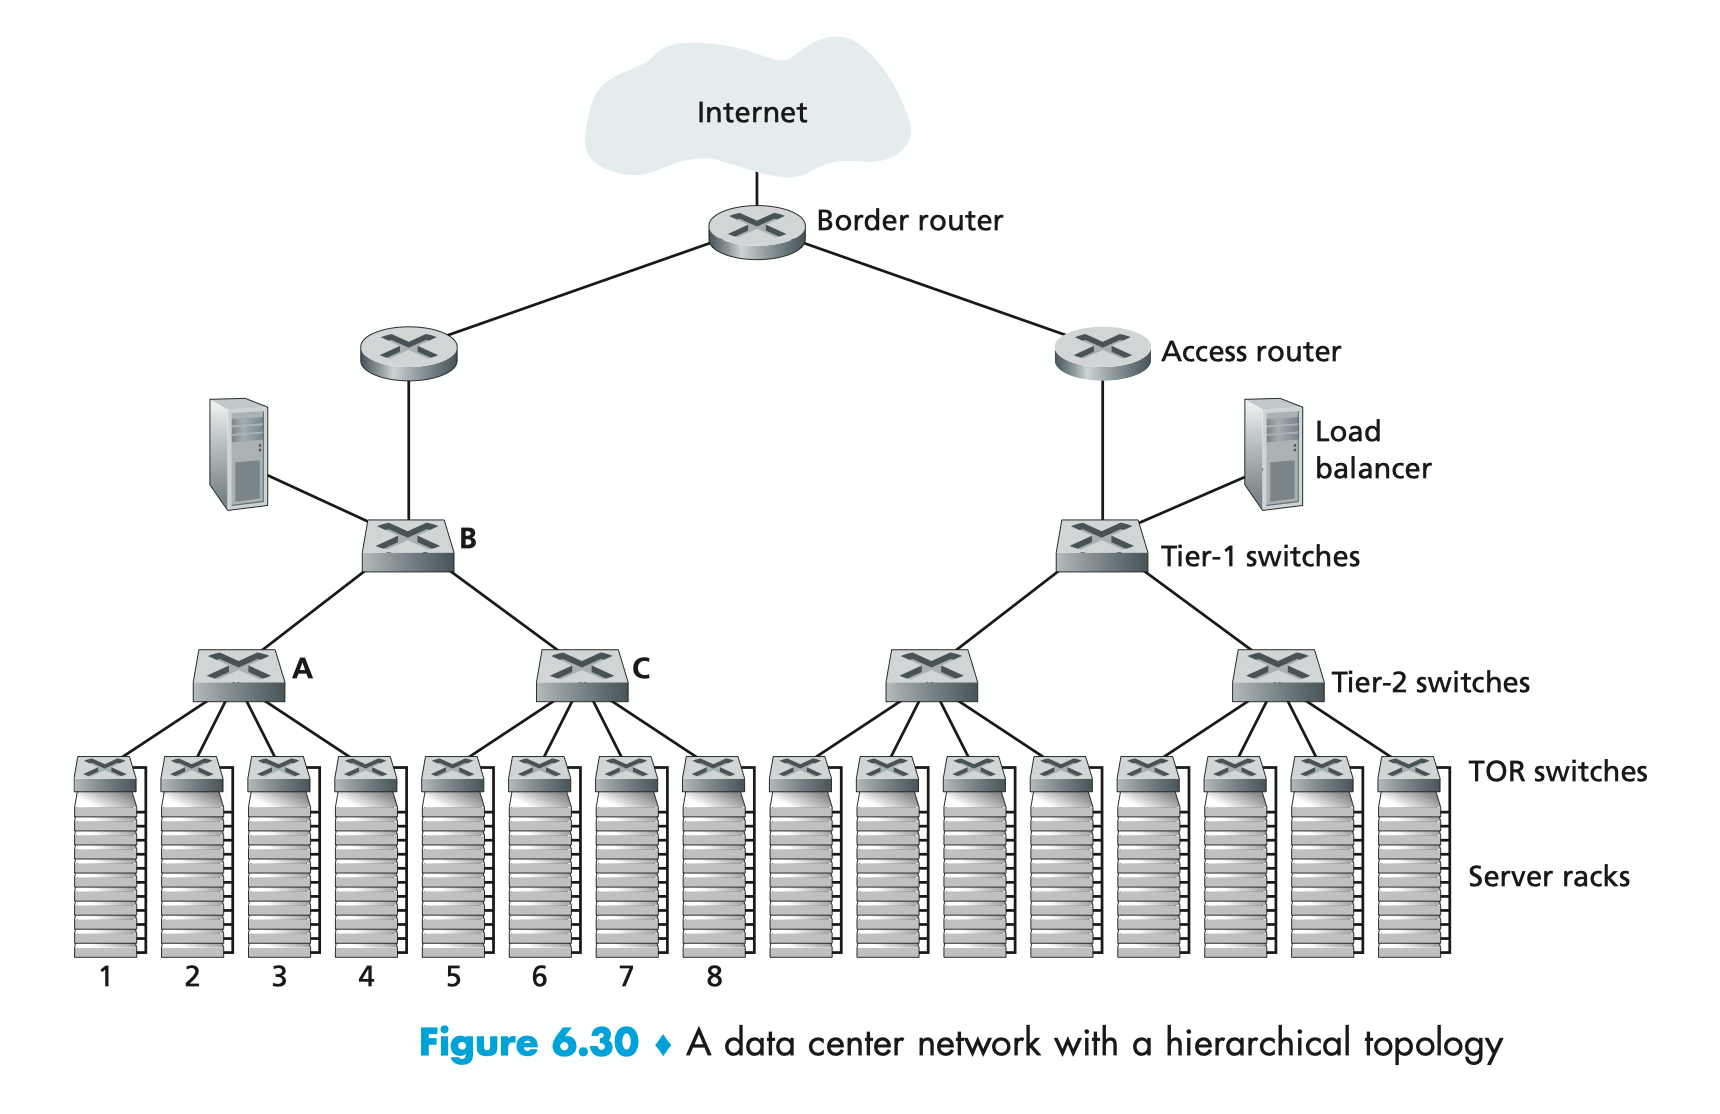
\includegraphics[width=0.85\textwidth]{Fig6.30.png}
        % \caption{}
        % \label{fig:I2Cdemo}
    \end{figure}
    \begin{enumerate}
        \item For what fraction of time does the e-mail application need to use a fourth rack? How about for the video application?
        \item Assuming e-mail usage and video usage are independent, for what fraction of time do (equivalently, what is the probability that) both applications need their fourth rack?
        \item Suppose that it is acceptable for an application to have a shortage of servers for 0.001 percent of time or less (causing rare periods of performance degradation for users). Discuss how the topology in Figure 6.31 can be used so that only seven racks are collectively assigned to the two applications (assuming that the topology can support all the traffic).
        \begin{figure}[h!]
            \centering
            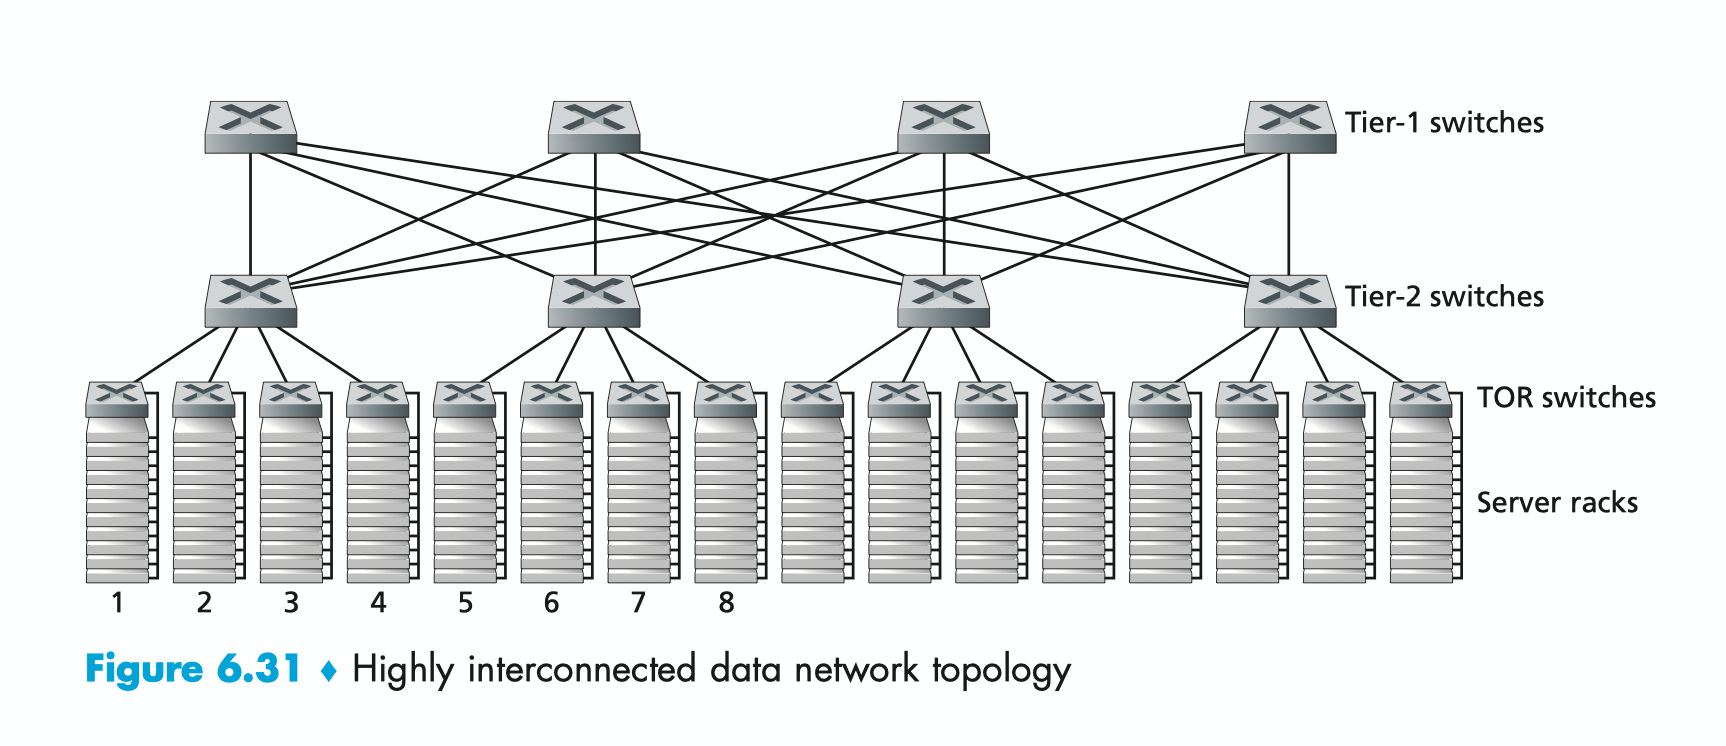
\includegraphics[width=0.85\textwidth]{Fig6.31.png}
            % \caption{}
            % \label{fig:I2Cdemo}
        \end{figure}
    \end{enumerate}
\end{enumerate}
\end{document}